\documentclass[a4paper,12pt,abstracton]{scrartcl}
\usepackage[utf8]{inputenc}
\usepackage{float}
\usepackage{tikz}
\usepackage{amsmath}
\usepackage{amssymb}
\usepackage{pifont}% http://ctan.org/pkg/pifont
\usepackage[font=small,labelfont=bf]{caption}
\usepackage{graphicx}
\usepackage{dirtytalk}
\usepackage{multicol}
\usepackage{booktabs}
\usepackage{colortbl}
\usepackage{appendix}
\usepackage{nomencl}
\usepackage{lmodern}
\usepackage[nottoc]{tocbibind}
\usepackage{xcolor}
%\graphicspath{images/}
\usepackage[margin = 3cm]{geometry}
\usepackage{ragged2e} % good alignment
\usepackage{hyperref}
\usepackage{siunitx} % Provides the \SI{}{} and \si{} command for typesetting SI units
\hypersetup{colorlinks=true,
    linkcolor=blue,
    filecolor=magenta,      
    urlcolor=cyan, 
    citecolor=gray}

%\DeclareGraphicsExtensions{.png,.pdf} % low-res (work in progress)
%\DeclareGraphicsExtensions{.pdf,.png}  % high-res (final draft)
%\setlength\parindent{0pt} % Removes all indentation from paragraphs
%\bibliographystyle{unstr}
\setlength\parindent{0pt}
\setlength{\parskip}{0.3em}
\newcommand{\xmark}{\ding{55}}

\begin{document}
\section{Appendix}\label{appendix}
The diffractograms are arranged according to the following rule: 
$$
\begin{tabular}{l l}
\textbf{Normal Transverse} &\hspace{1cm} \textbf{Normal Longitudinal} \\ \\ 
\textbf{Anomalous Transverse}  &\hspace{1cm} \textbf{Anomalous Longitudinal} 
\end{tabular}
$$

\begin{figure}[H]
    \centering
    \begin{tabular}{c c}
      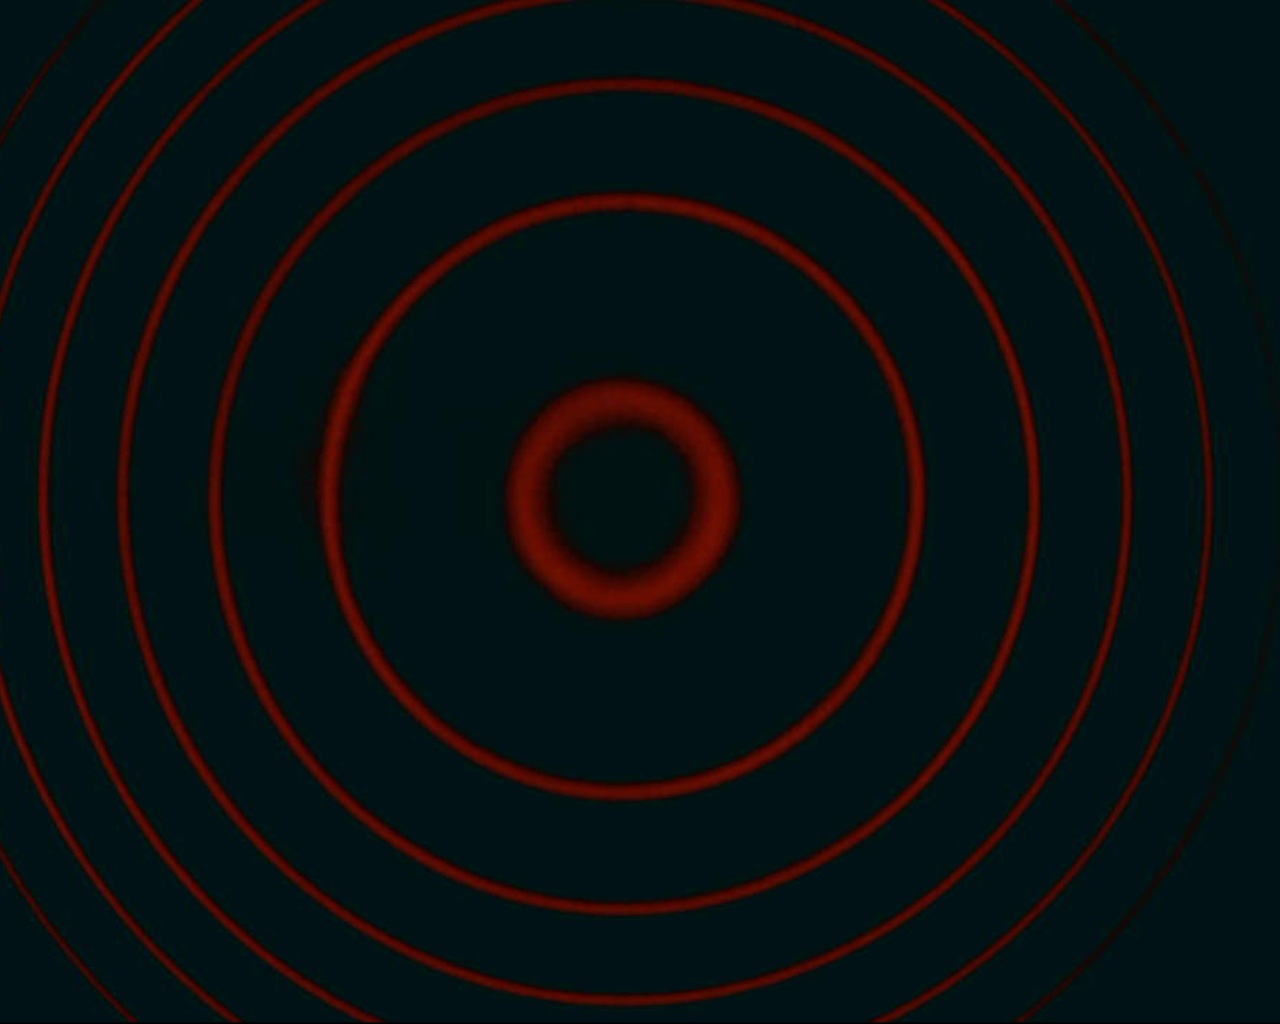
\includegraphics[height=6cm,keepaspectratio]{images/z0.png} & 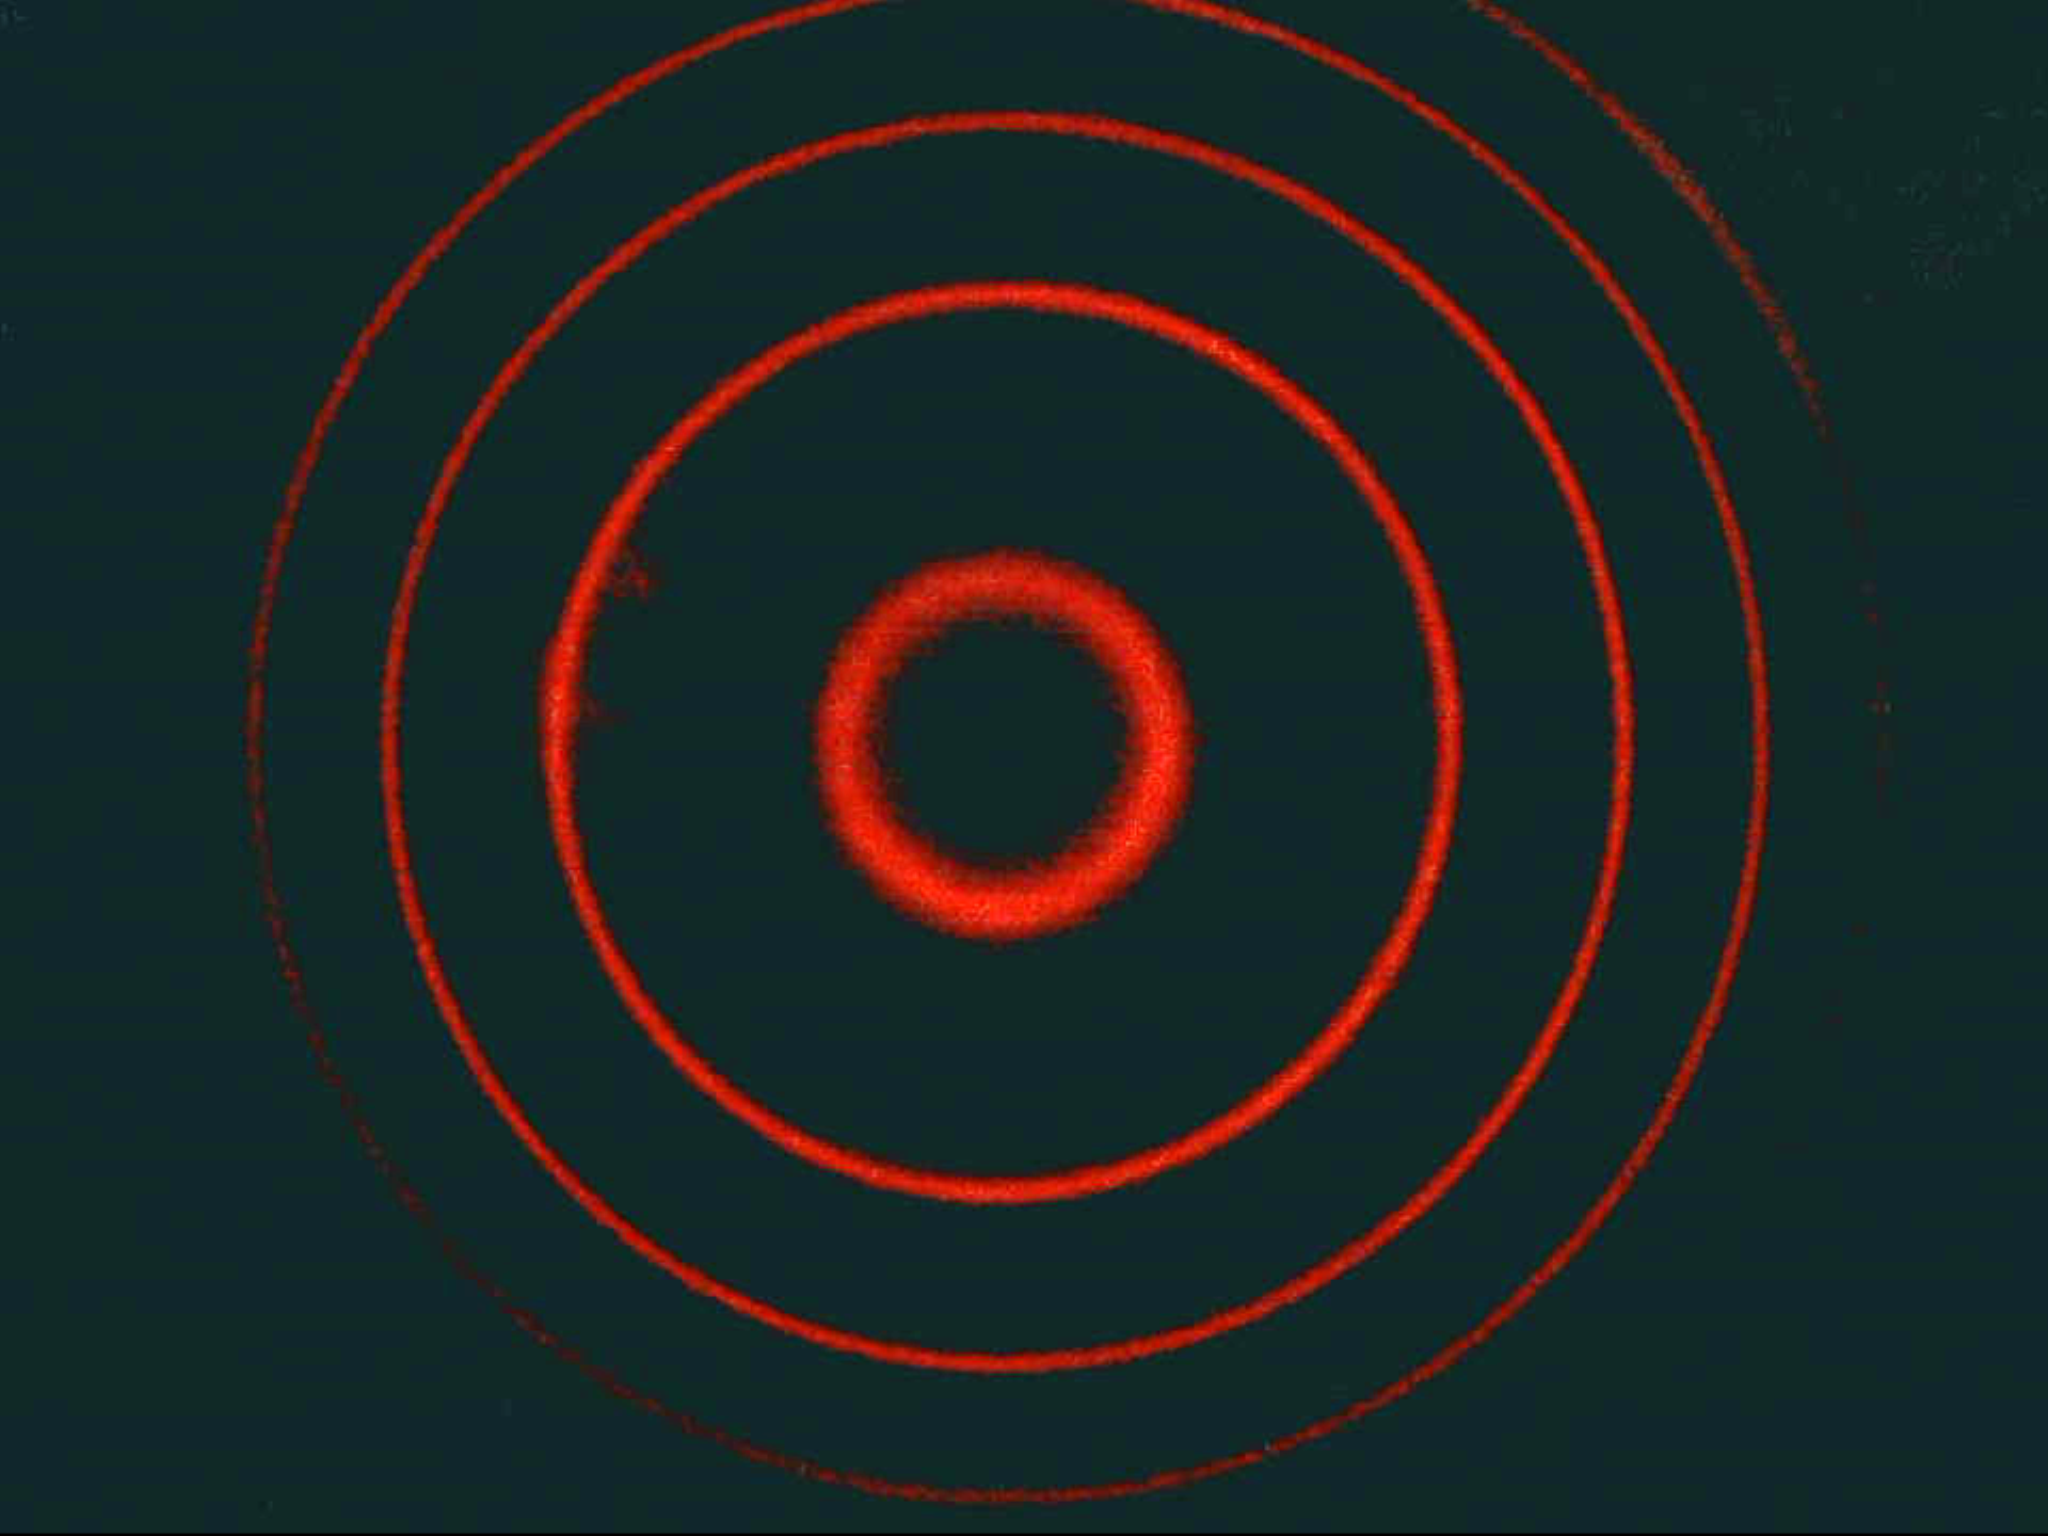
\includegraphics[height=6cm,keepaspectratio]{images/zl0.png} \\\\
      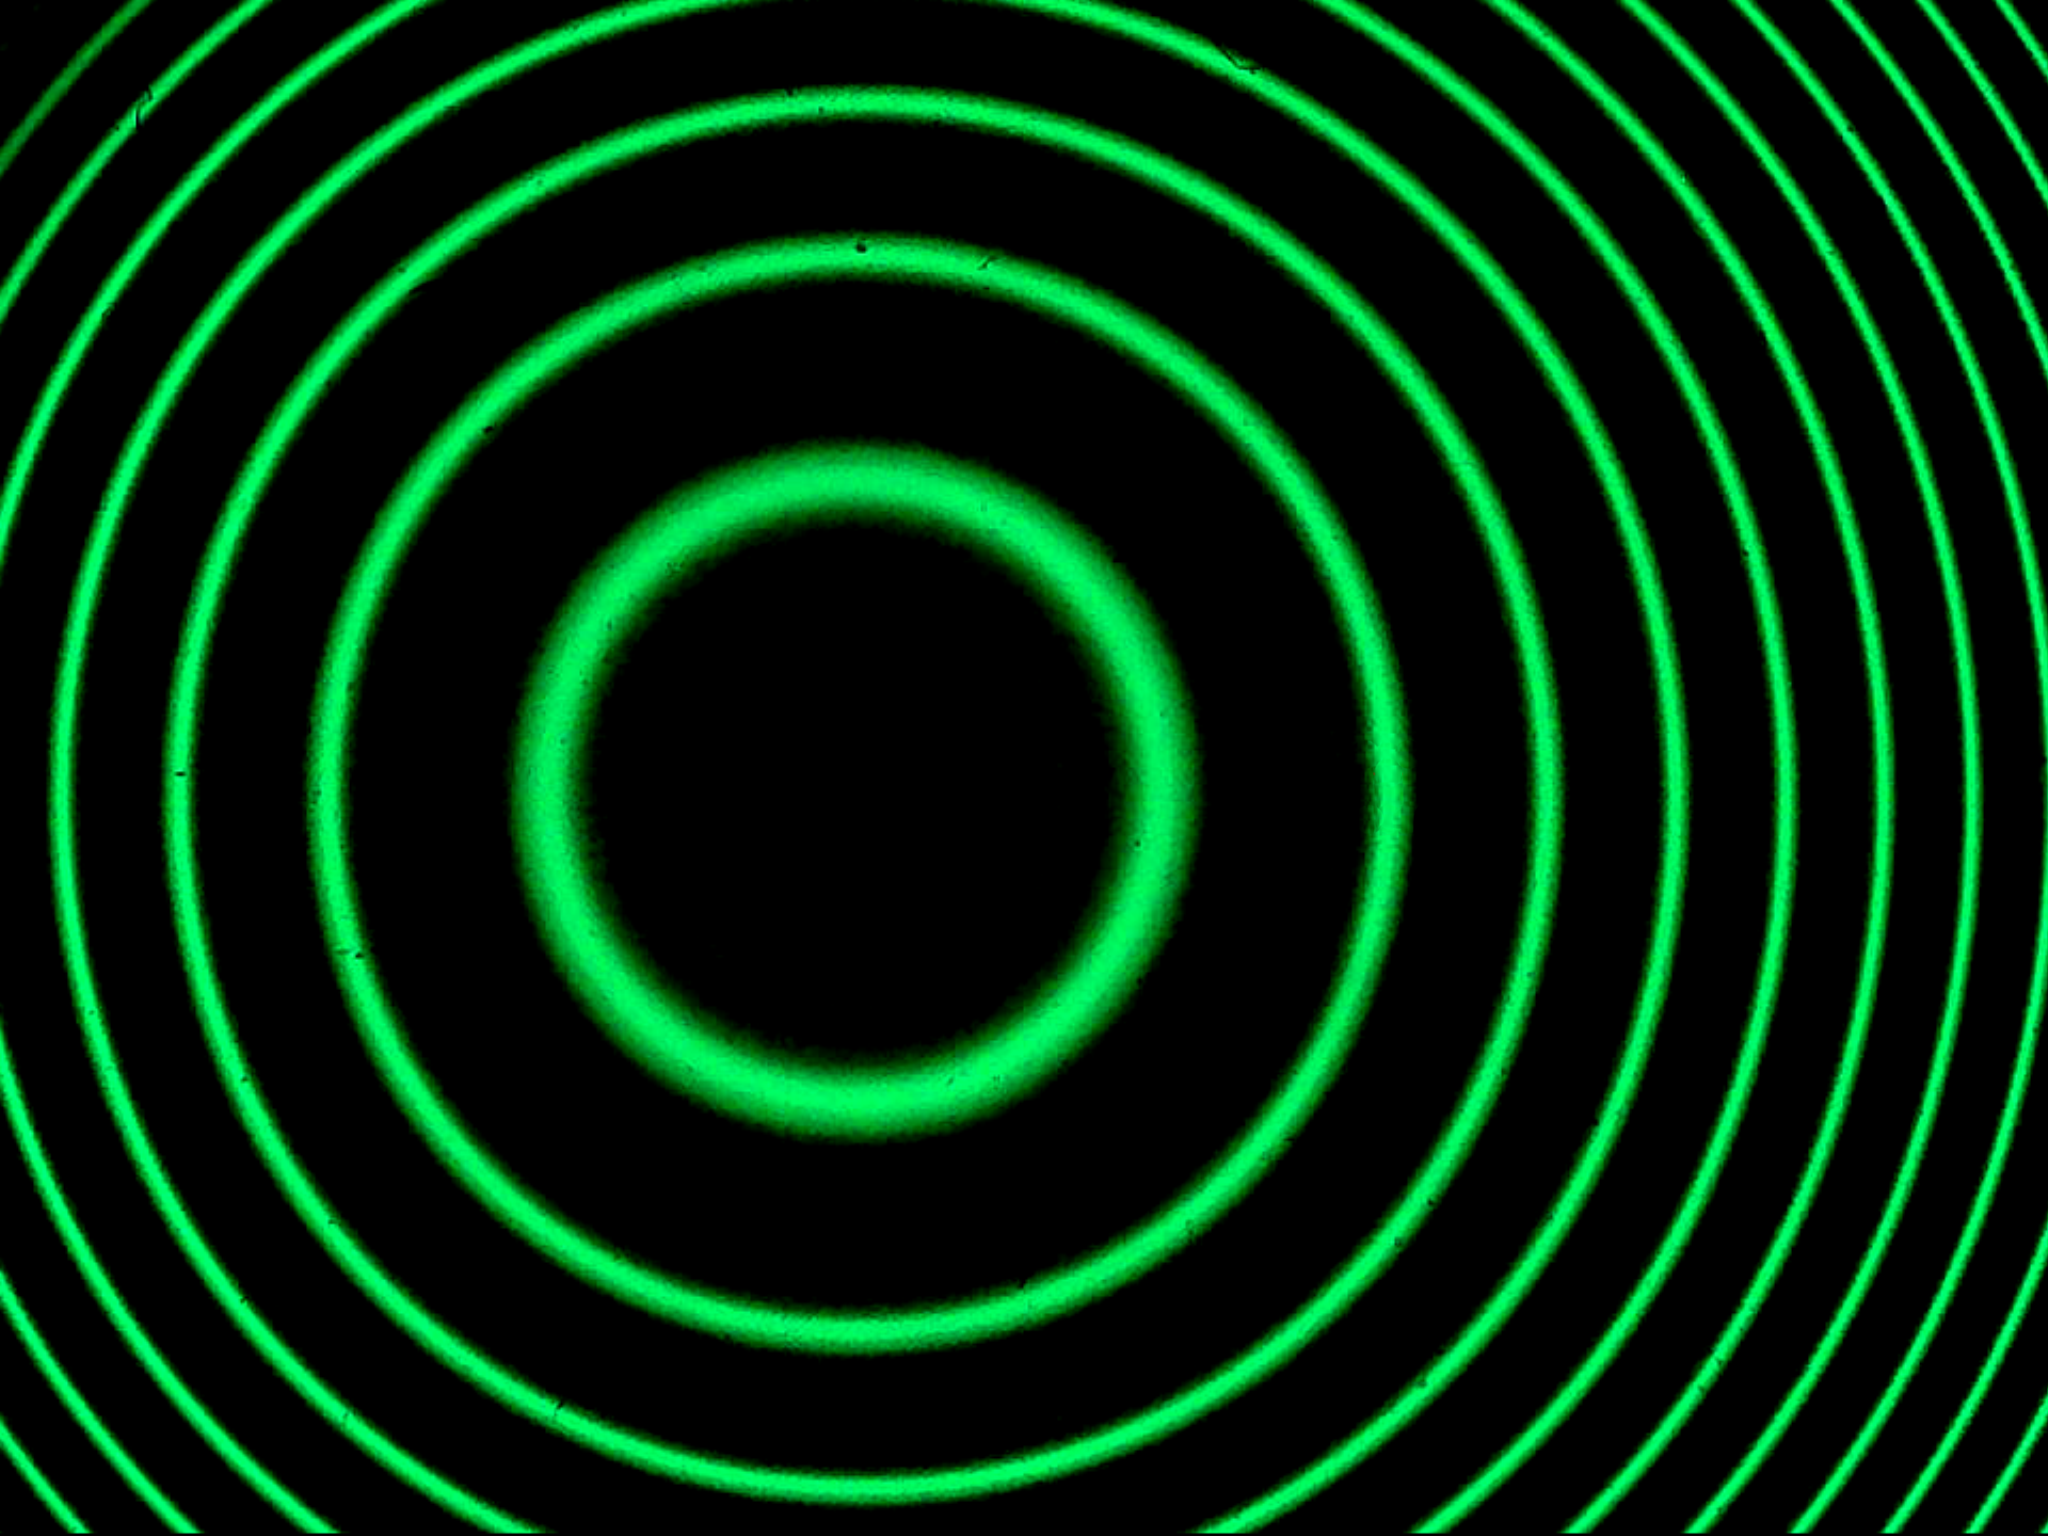
\includegraphics[width=7.5cm,keepaspectratio]{images/za0.png} & 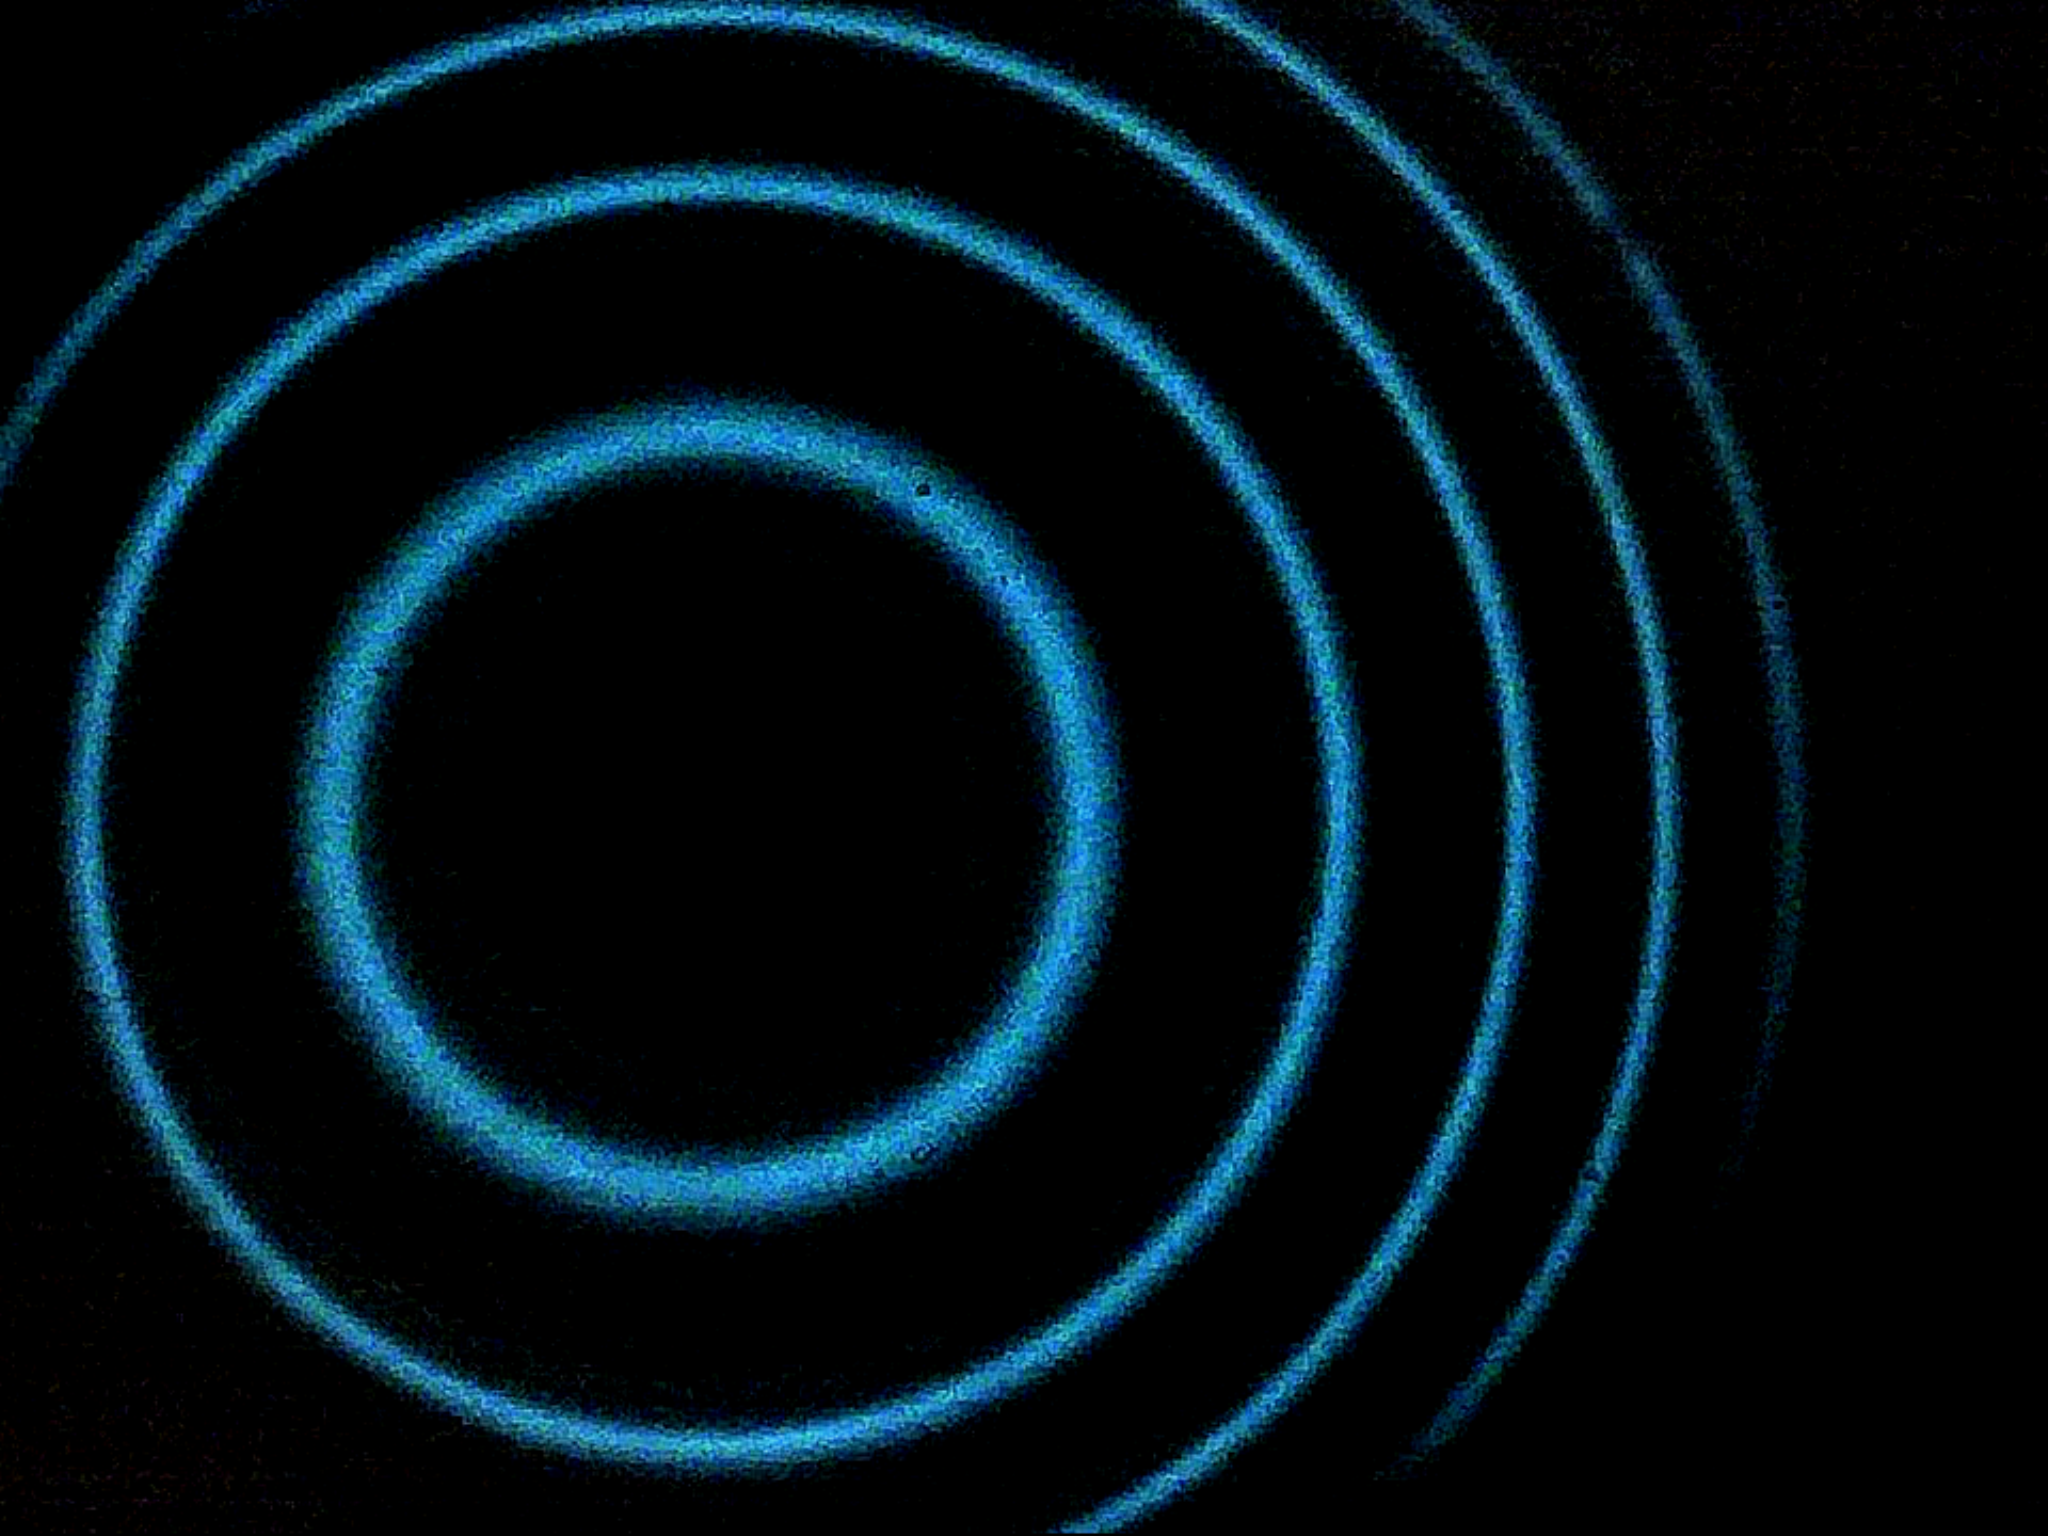
\includegraphics[height=6cm,keepaspectratio]{images/zal0.png} \\
      \end{tabular}
    \caption{$B=0$ T }
    \label{fig:B0}
\end{figure}

\begin{figure}[H]
    \centering
    \begin{tabular}{c c}
      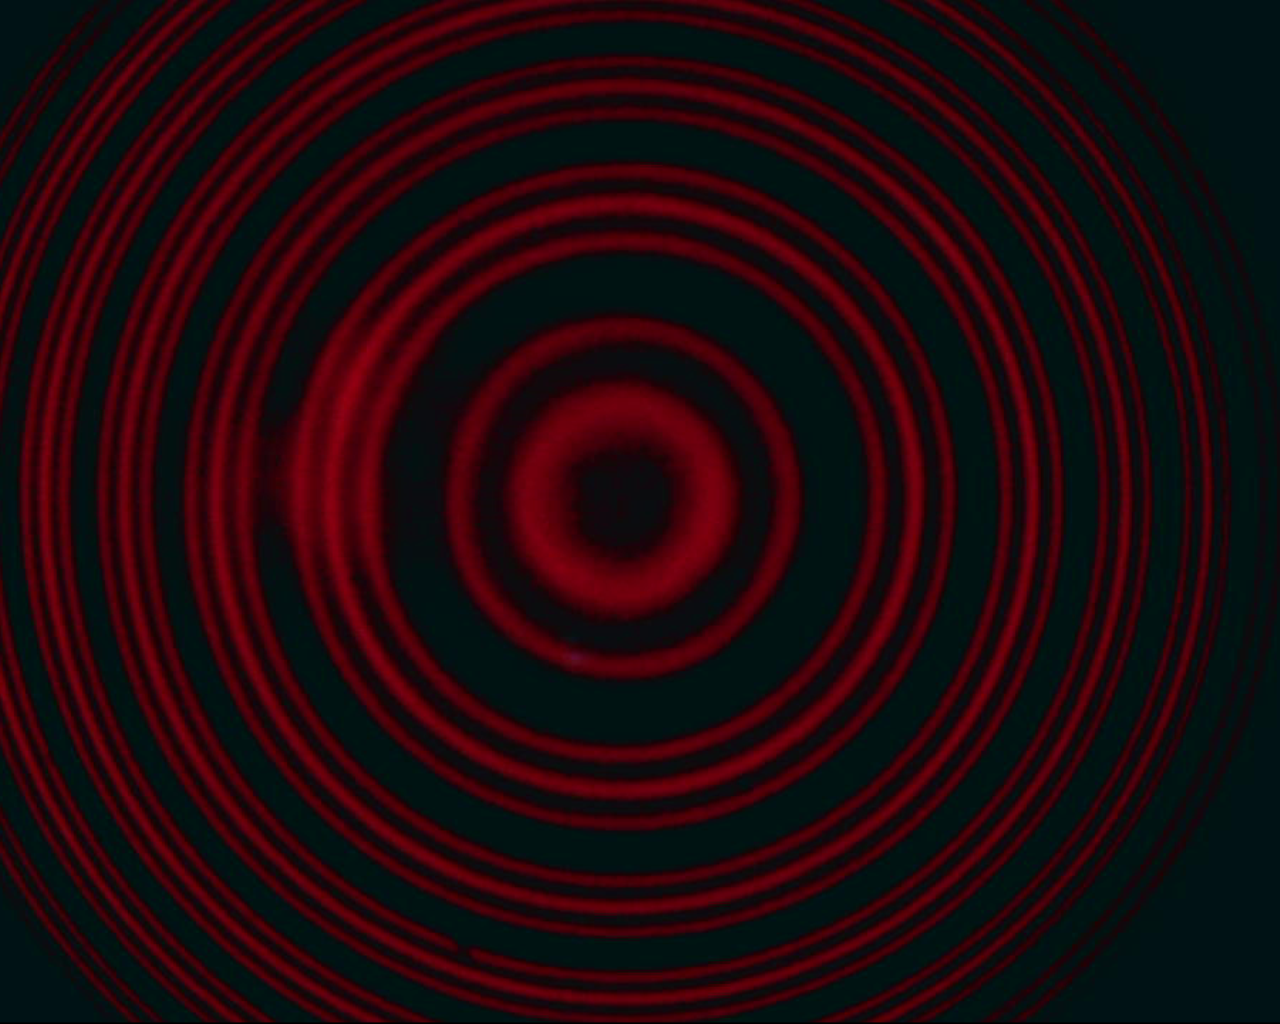
\includegraphics[height=6cm,keepaspectratio]{images/zn5.png} & 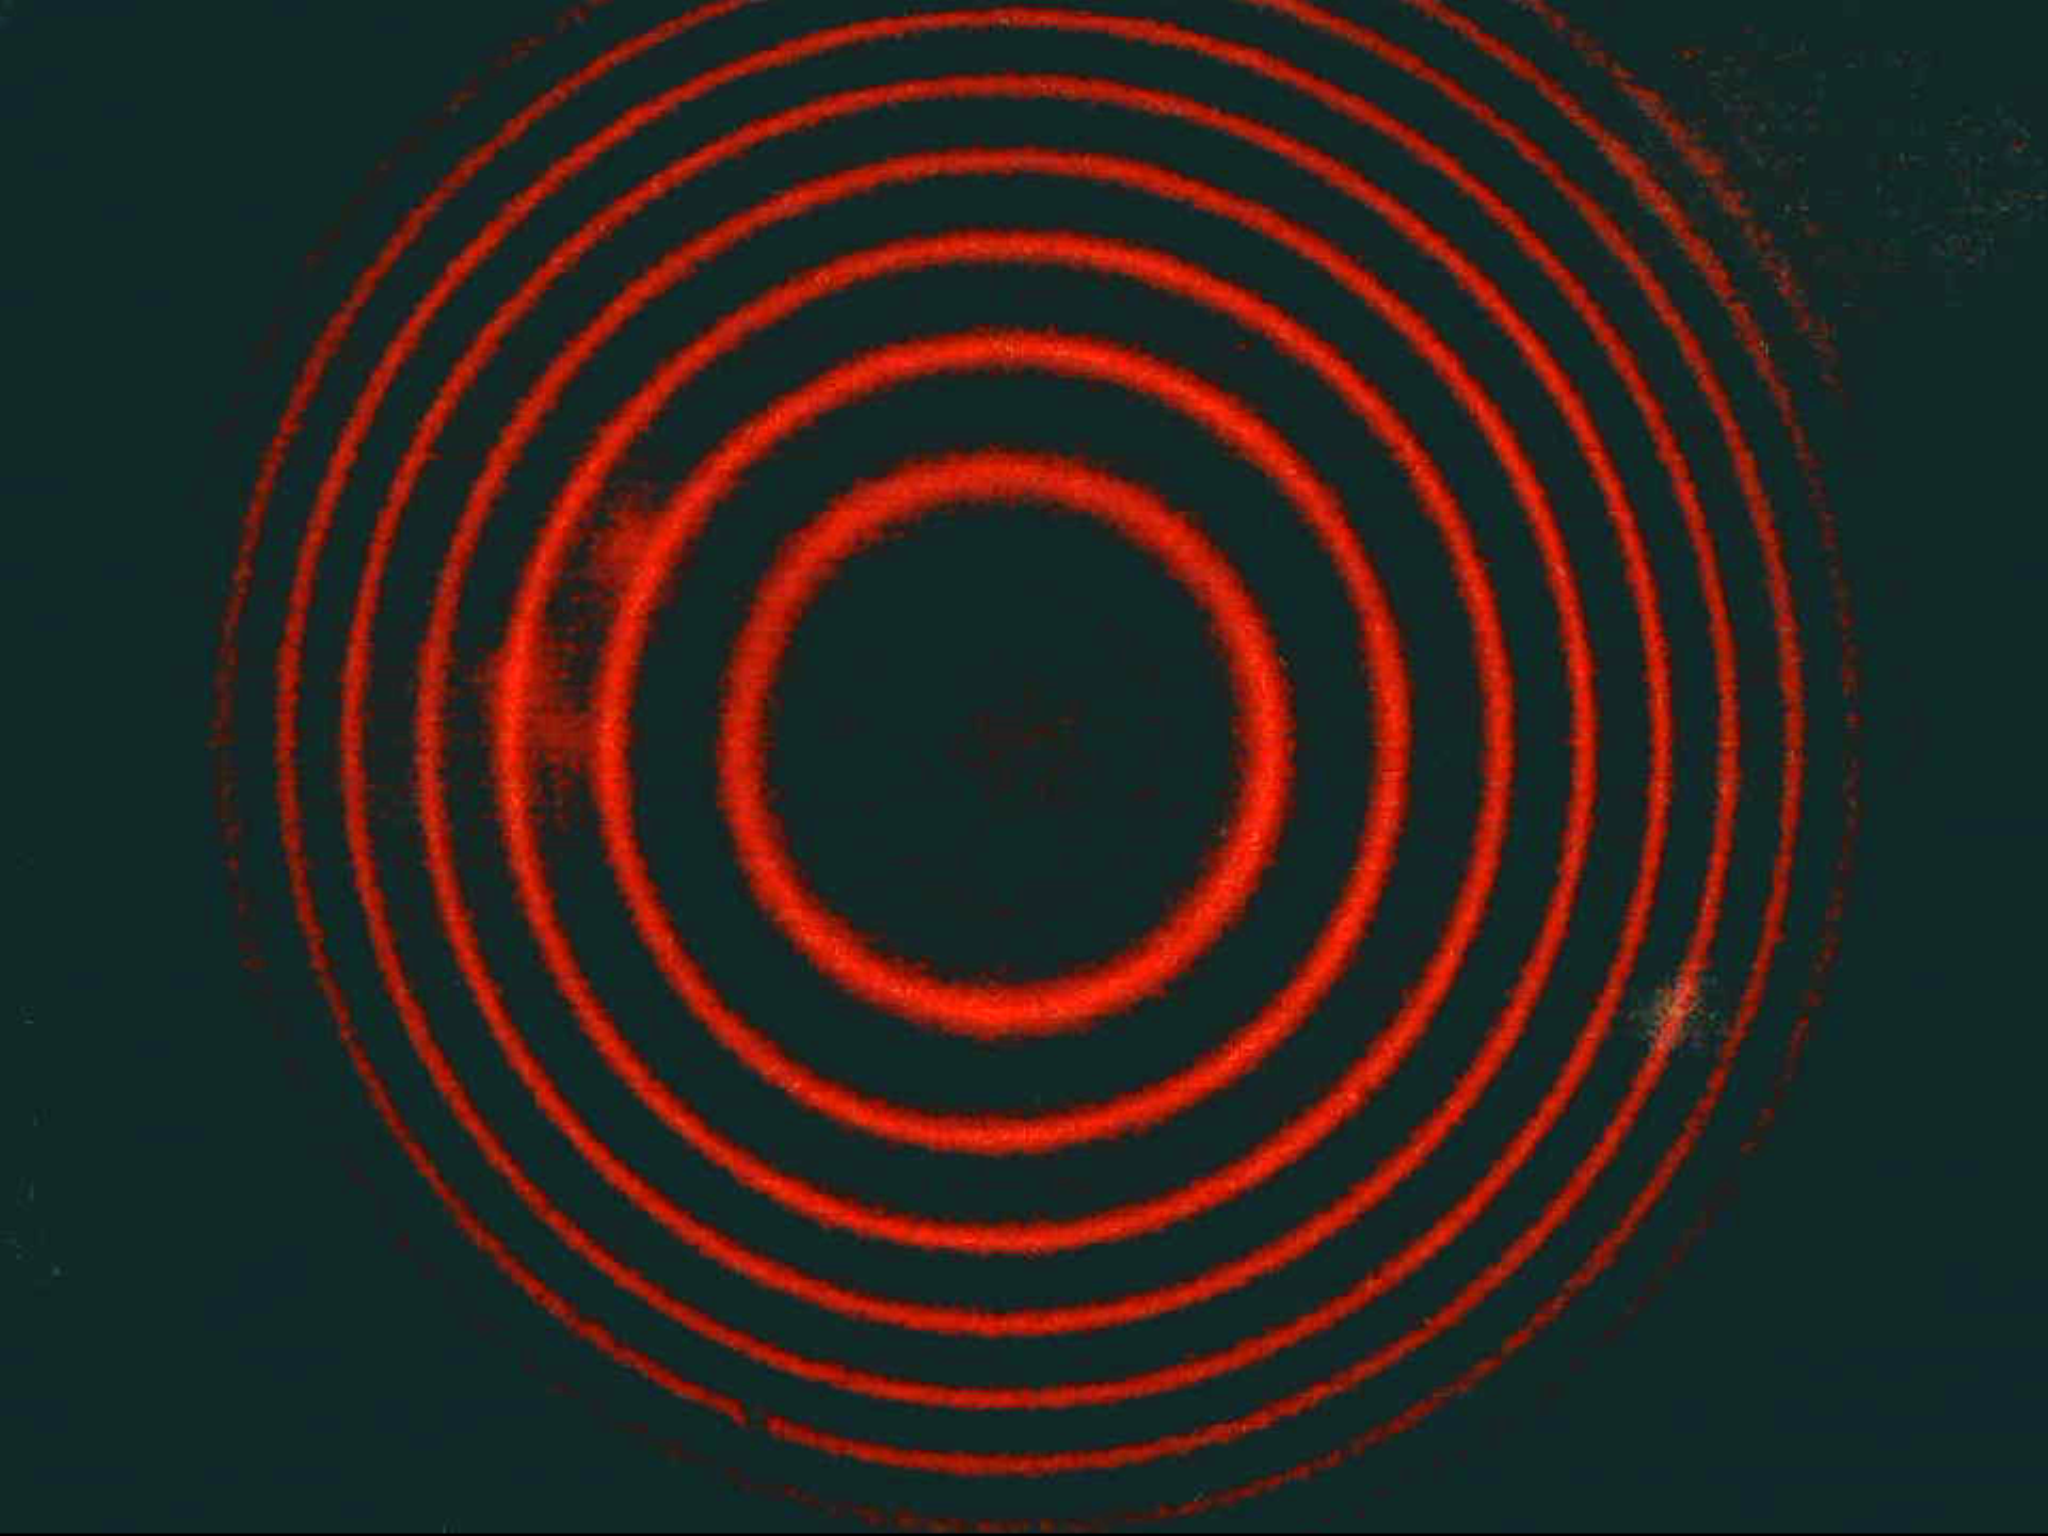
\includegraphics[height=6cm,keepaspectratio]{images/znl8.png} \\
      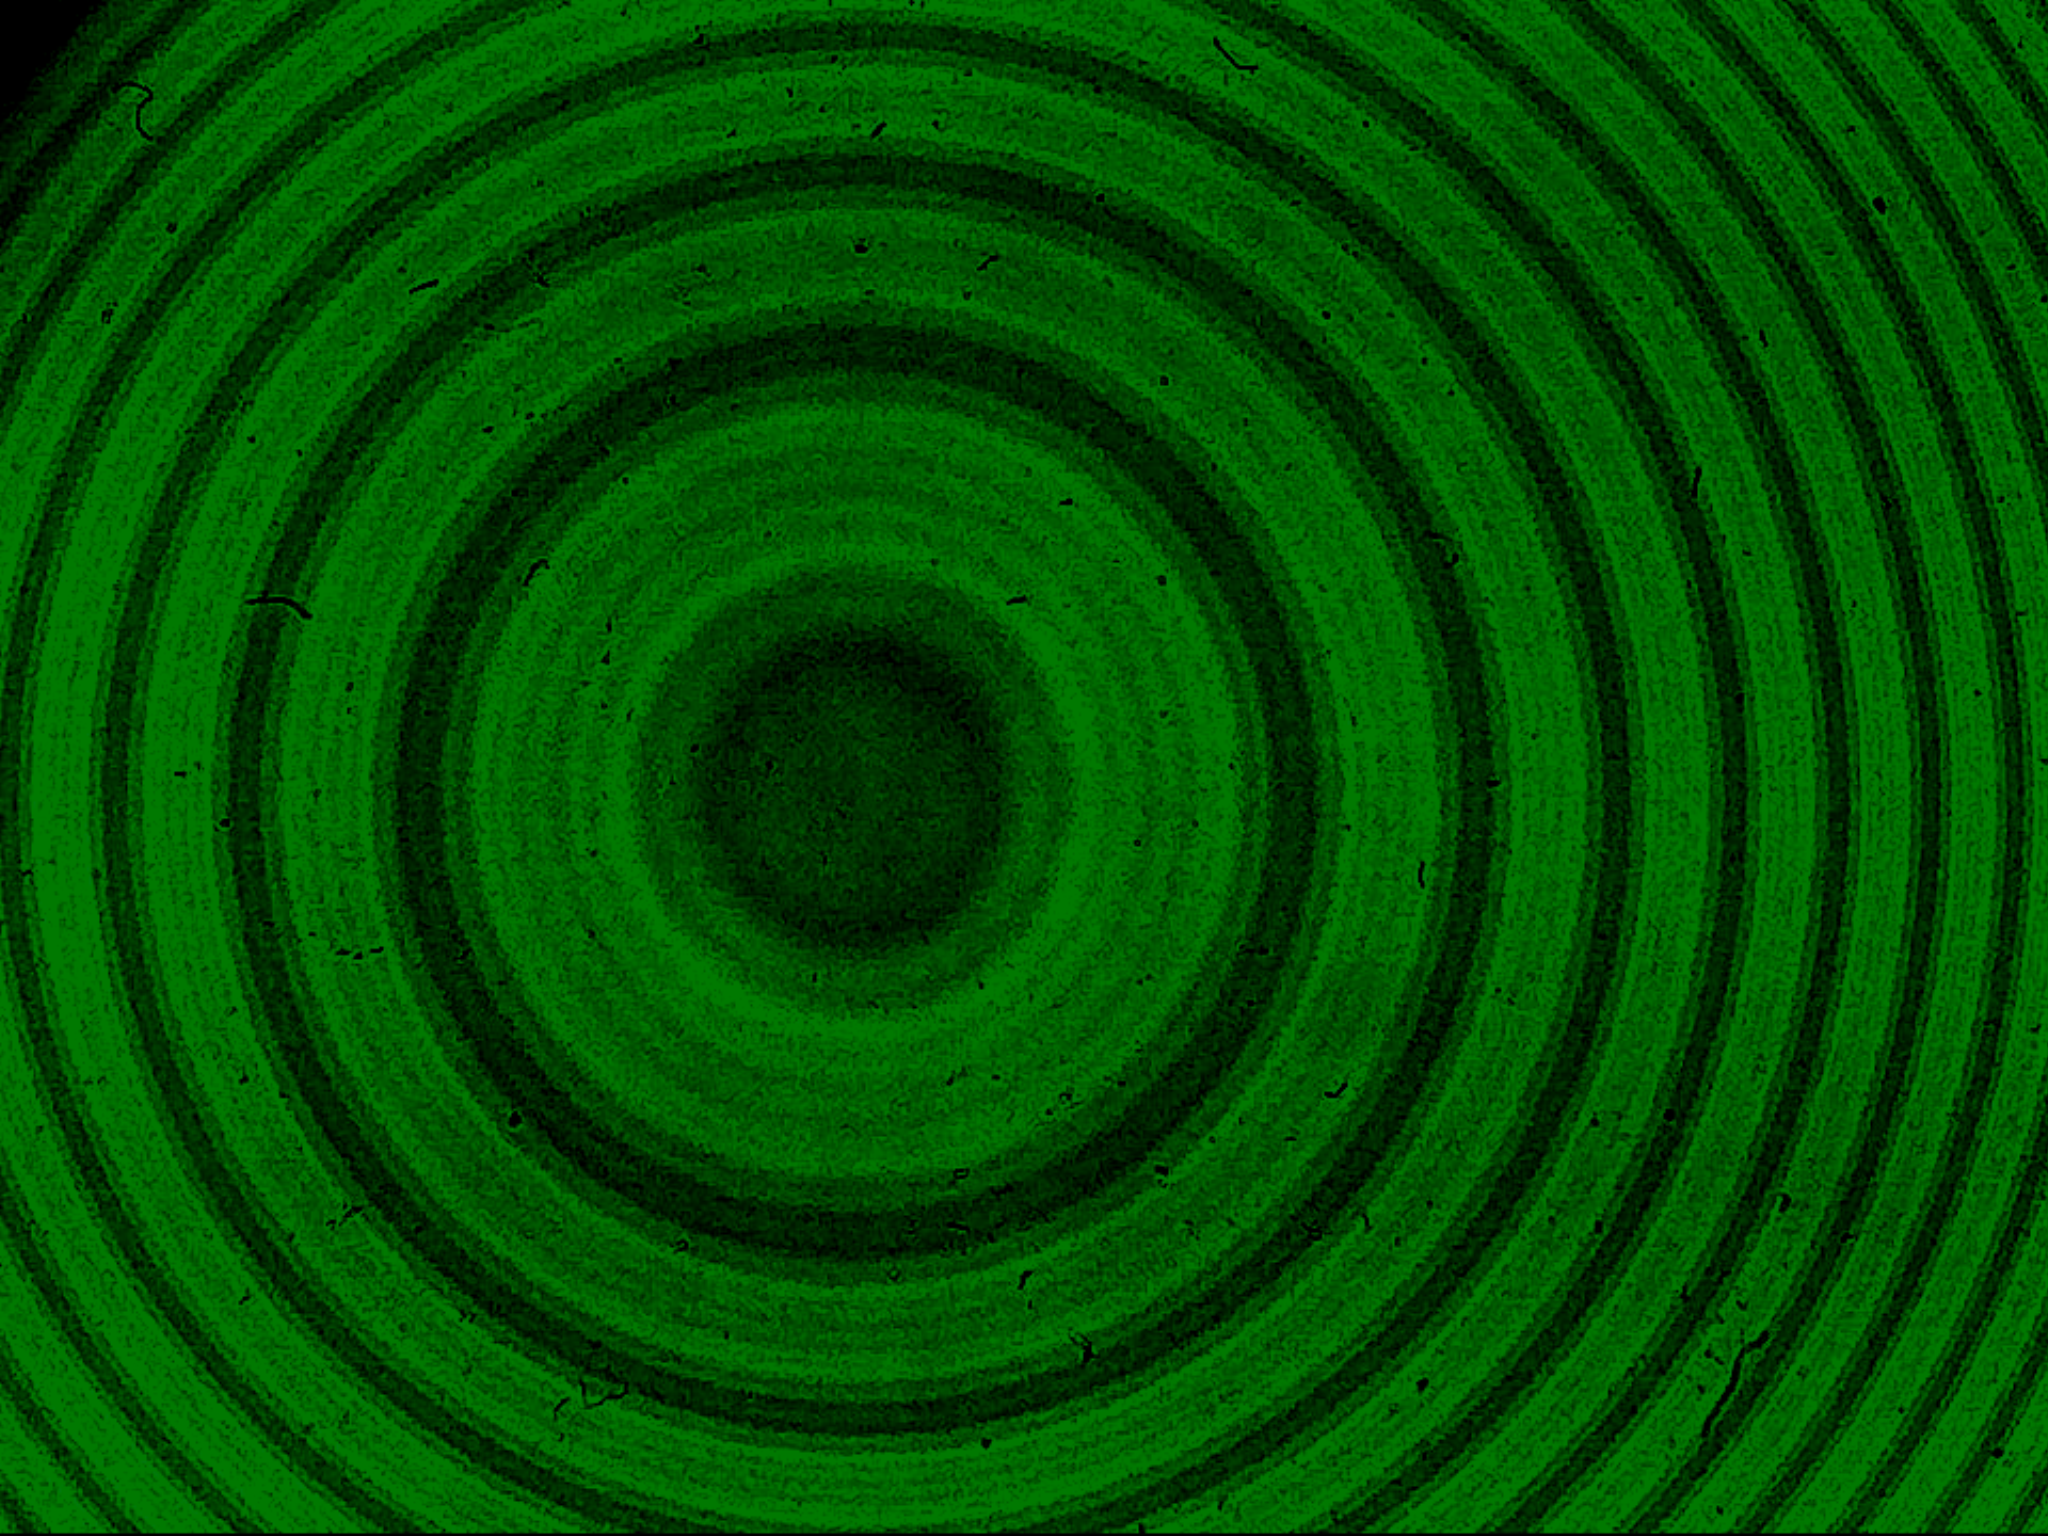
\includegraphics[width=7.5cm,keepaspectratio]{images/za4.png} & \includegraphics[height=6cm,keepaspectratio]{images/zal5.png} \\
      \end{tabular}
    \caption{No Polarization }
    \label{fig:np}
\end{figure}

\begin{figure}[H]
    \centering
    \begin{tabular}{c c}
      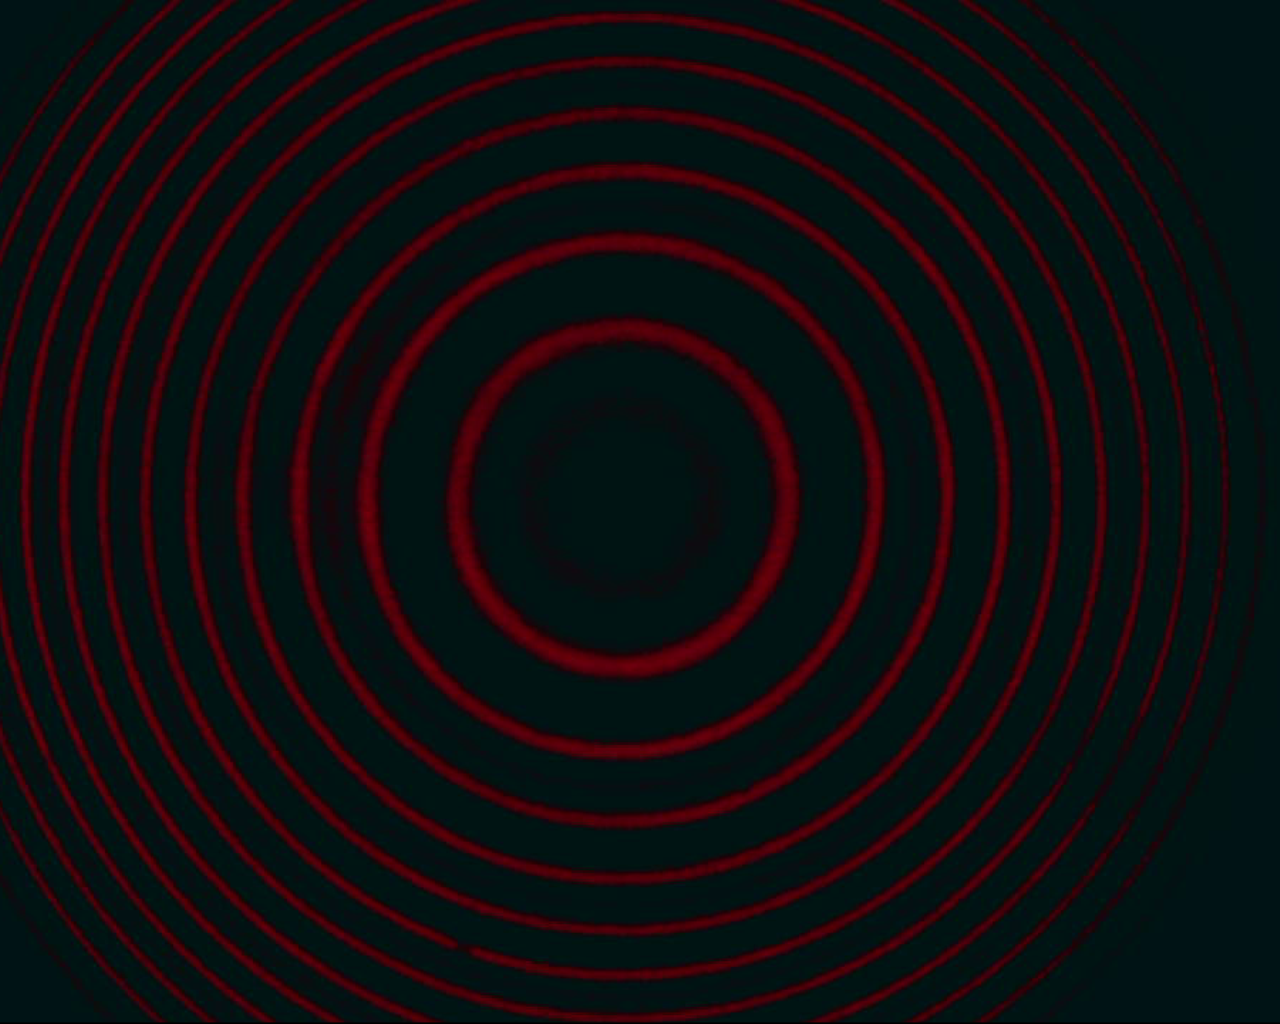
\includegraphics[height=6cm,keepaspectratio]{images/zna5.png} & 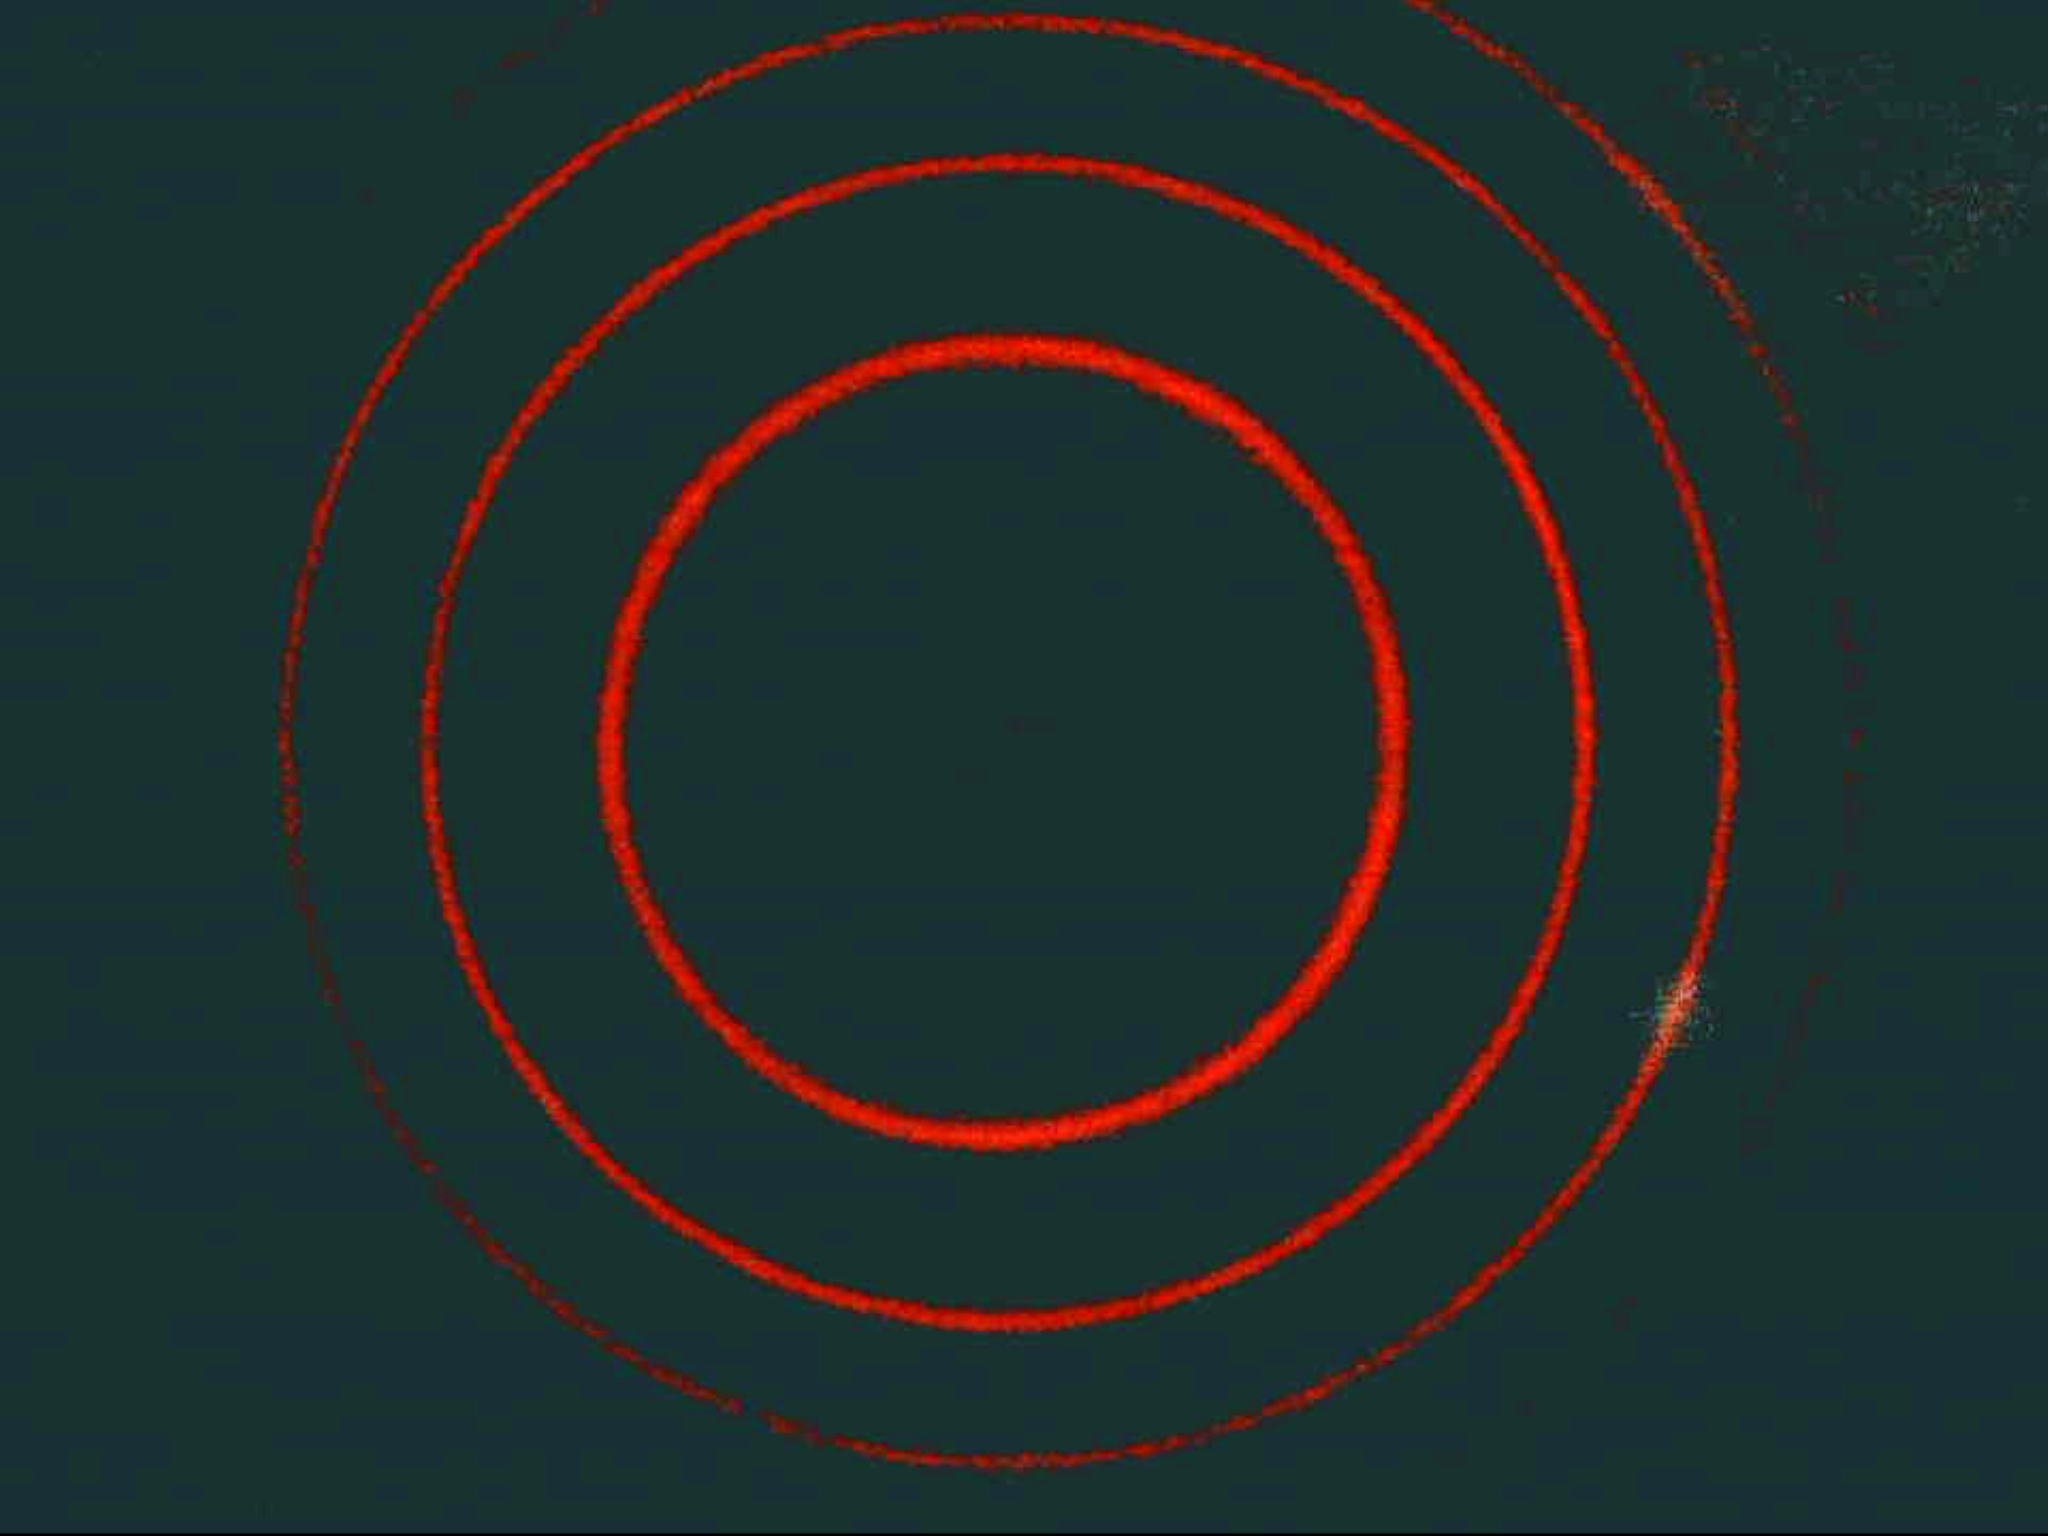
\includegraphics[height=6cm,keepaspectratio]{images/znla8.png} \\
      \includegraphics[width=7.5cm,keepaspectratio]{images/zaa4.png} & \includegraphics[height=6cm,keepaspectratio]{images/zala5.png} \\
      \end{tabular}
    \caption{Polarization $a$}
    \label{fig:pa}
\end{figure}

\begin{figure}[H]
    \centering
    \begin{tabular}{c c}
      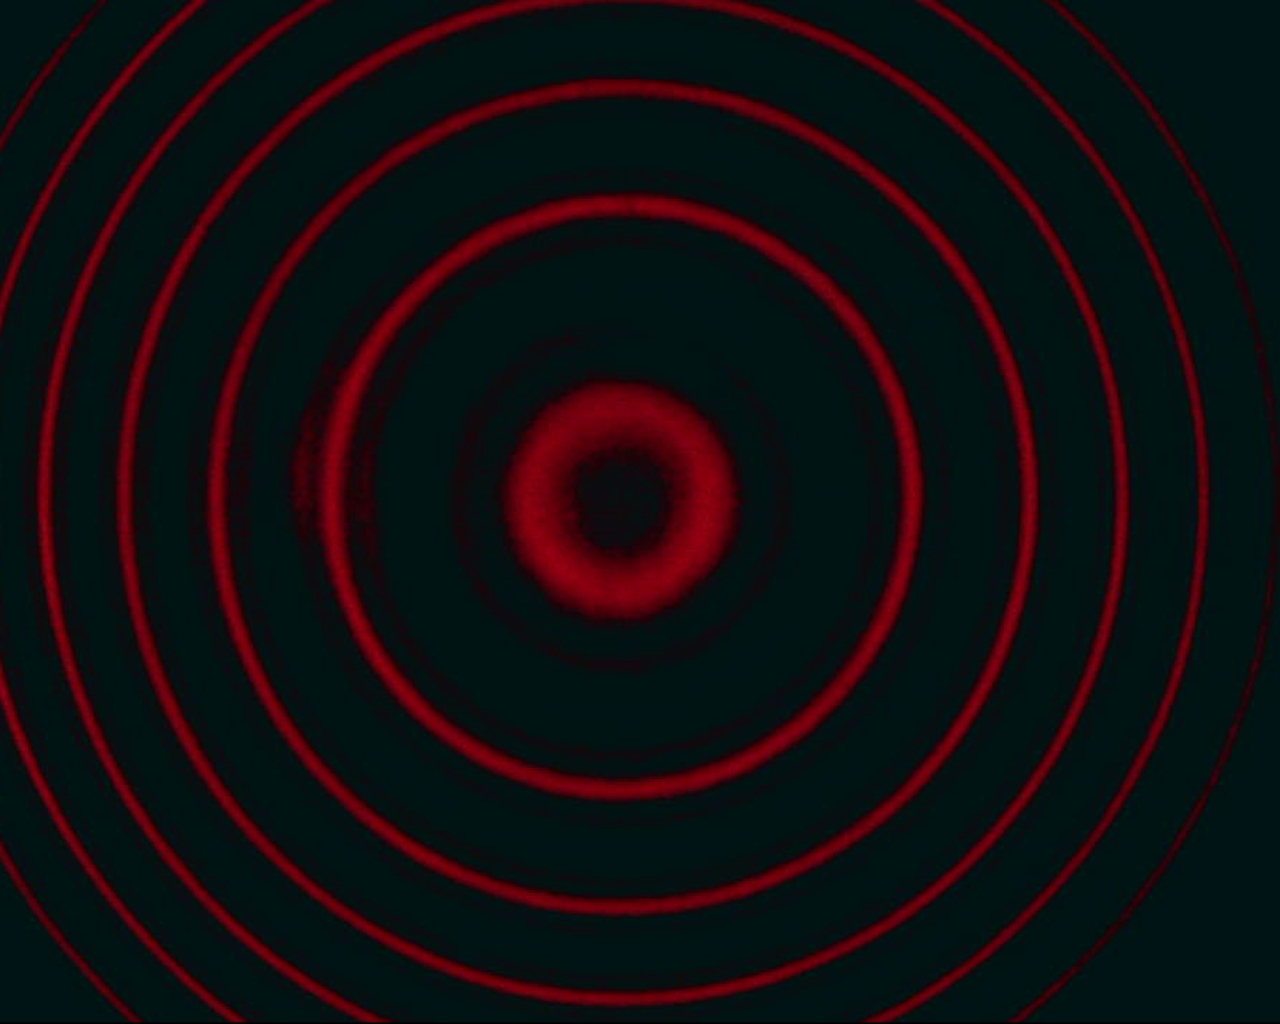
\includegraphics[height=6cm,keepaspectratio]{images/znb5.png} & 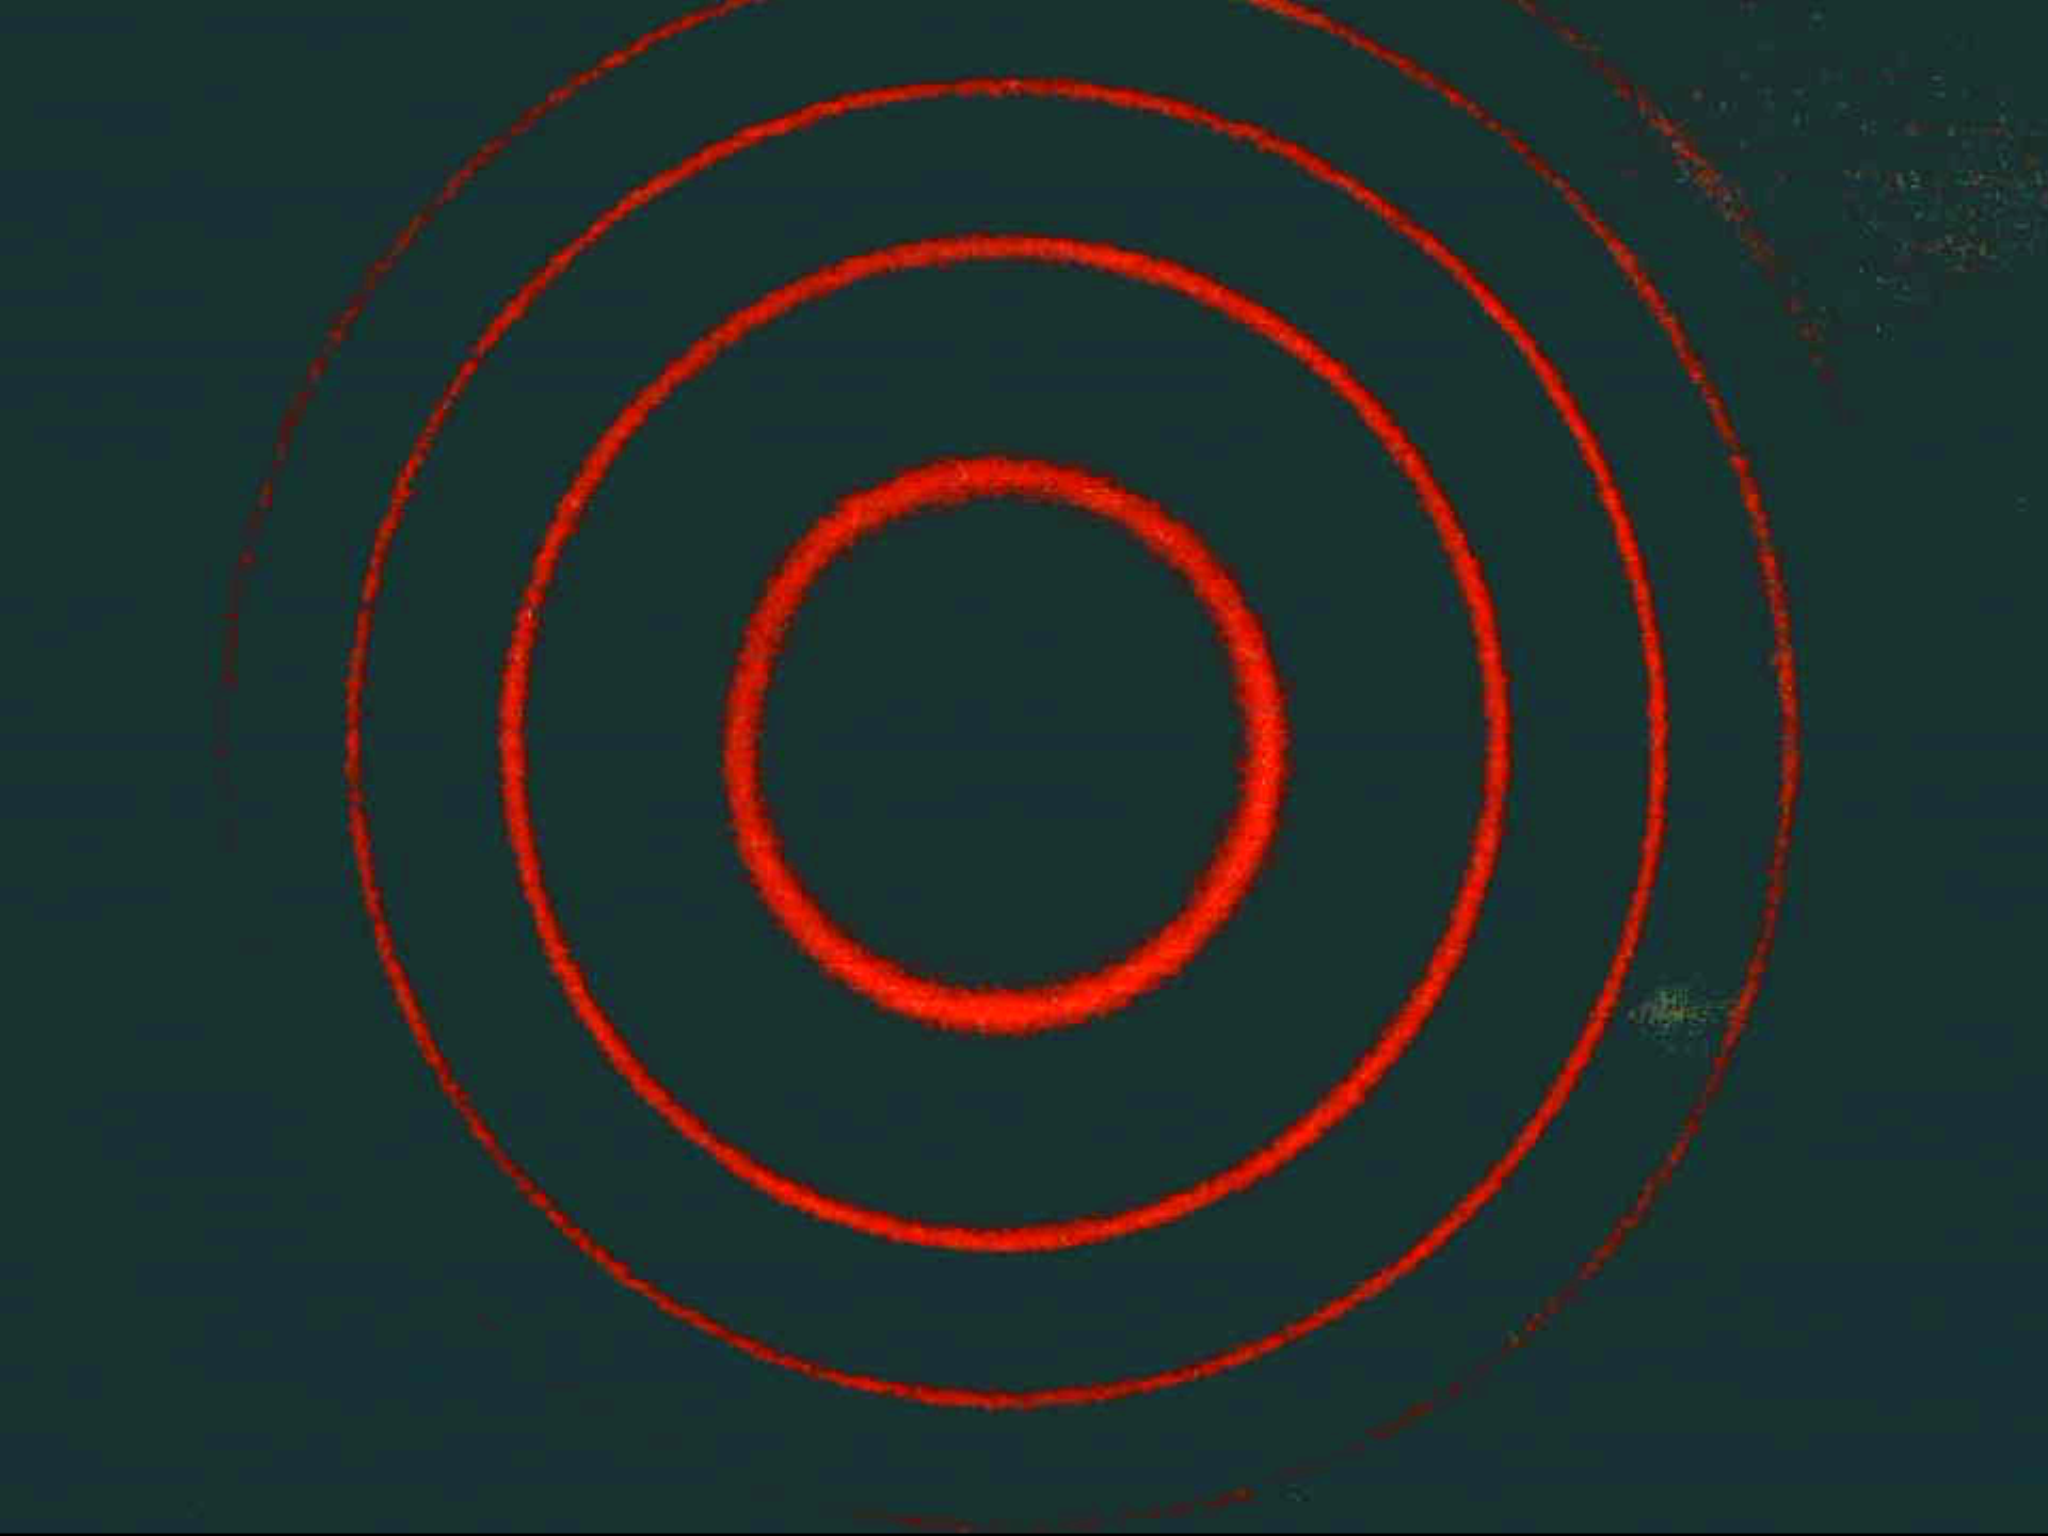
\includegraphics[height=6cm,keepaspectratio]{images/znlb8.png} \\
      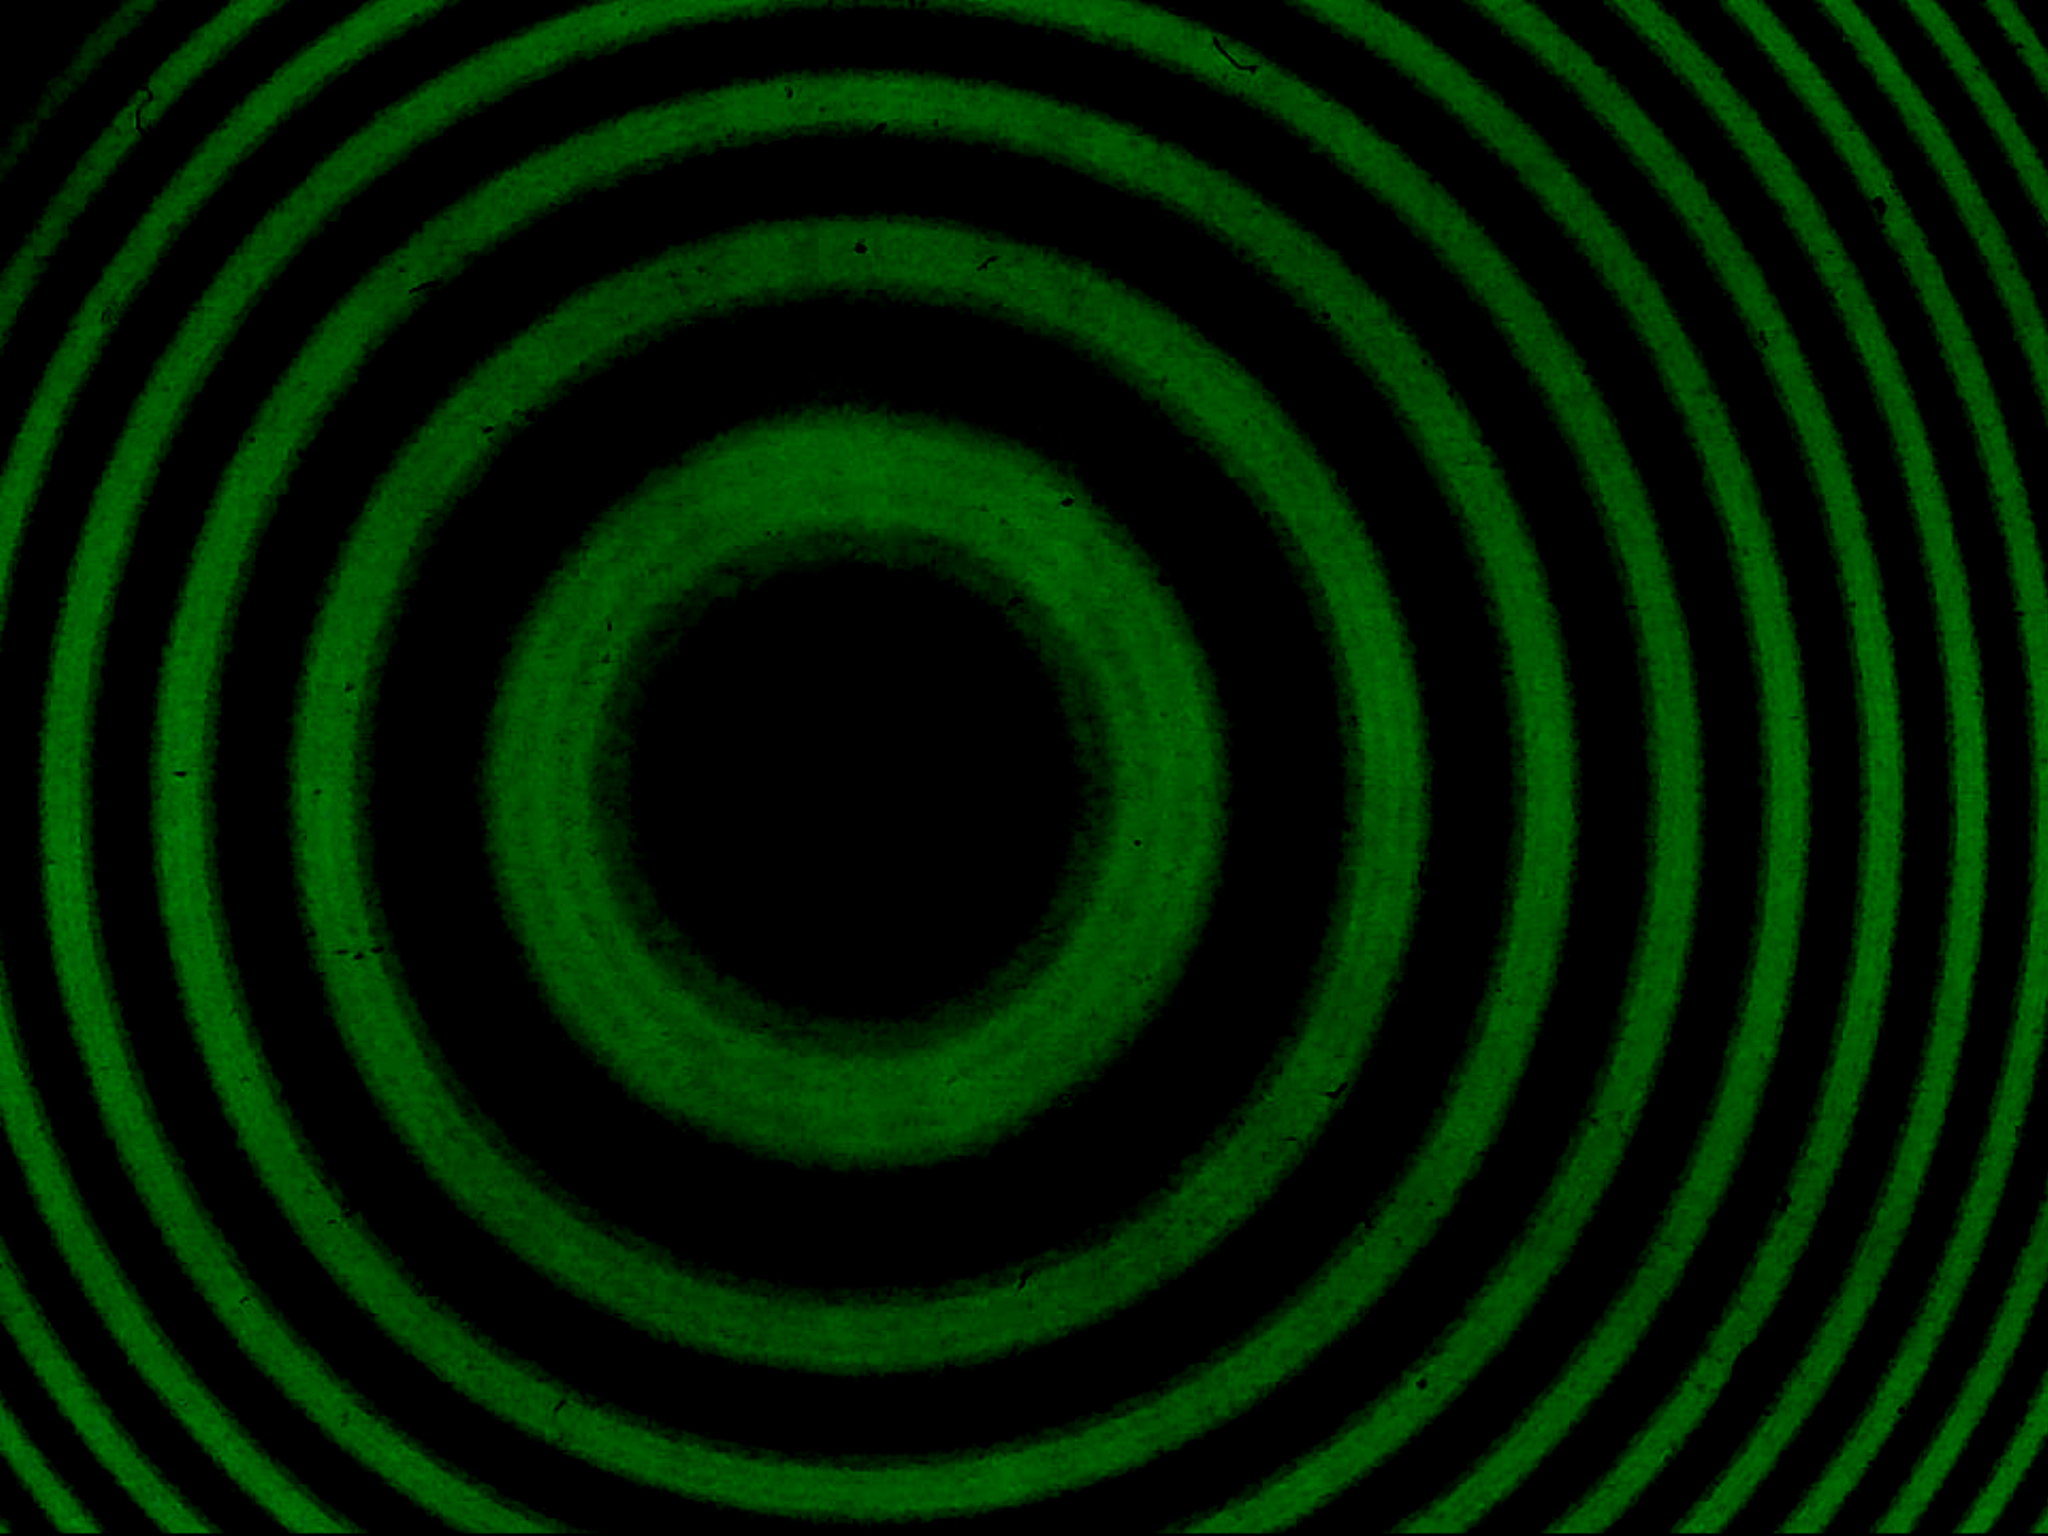
\includegraphics[width=7.5cm,keepaspectratio]{images/zab4.png} & \includegraphics[height=6cm,keepaspectratio]{images/zalb5.png} \\
      \end{tabular}
    \caption{Polarization $b$}
    \label{fig:pb}
\end{figure}

\end{document}